\chapter{Pruebas Estadísticas}


\section*{Contenido}
\begin{enumerate}
\item Introducción.
\item Características de la Distribución Uniforme.
\item Prueba de Promedio.
\item Prueba de Variancia.
\item Prueba de Corridas.
\item Prueba de Huecos con Dígitos.
\item Prueba de Huecos con Números.
\item Prueba de Póker.
\item Prueba de Series.
\item Resumen.
\item Ejercicios.
\end{enumerate}



\section{Introducción}


Dentro de un modelo de simulación la generación de cualquier variable no uniforme, es decir, normal, exponencial, poisson, etc, se obtiene a partir de números uniformes. Por ello se brinda especial énfasis a las pruebas estadísticas para números pseudoaleatorios, ya que cualquier deficiencia estadística en la distribución de la variable aleatoria se deberá exclusivamente a la utilización de un generador uniforme deficiente. 

En el presente capítulo se estudiarán algunas pruebas para determinar la eficiencia de un generador de números aleatorios.




\section{Características de la Distribución Uniforme}


La distribución uniforme suele representarese como:

$$f(x) =
\begin{cases} 
1 & \text{si } 0 \leq x \leq 1 \\
0 & \text{en otro caso}  
\end{cases}$$
        
La distribución acumulada está dada por:
$$F(x)=\int_{0}^{x} 1 \, dt$$
La integral de la constante $1$ con respecto a $t$ es:

$$\int 1 \, dt = t + C$$

donde $C$ es la constante de integración.

Ahora evaluamos la integral definida de $0$ a $x$:
$$F(x) = \left[ t \right]_{0}^{x}$$

Esto significa que sustituimos $t$ por $x$ y luego por $0$:
$$F(x) = x - 0$$

Por lo tanto, el resultado de la integral es:
$$F(x) = x$$

Por lo tanto:

$$F(x) =
\begin{cases} 
0 & \text{si } x \leq 0\\
x & \text{si } 0 \leq x \leq 1 \\
1 & \text{si } x \geq 1  
\end{cases}$$

A continuación se muestra de forma gráfica las funciones que se han obtenido.


\begin{center}
\begin{minipage}{0.45\textwidth} % Primer gráfico
    \begin{tikzpicture}[scale=4] % Escala de 4 cm por unidad
        % Ejes
        \draw[->] (-0.2,0) -- (1.2,0) node[right] {$x$};
        \draw[->] (0,-0.2) -- (0,1.2) node[above] {$y$};

        % Gráfico de f(x)
        \draw[blue, thick] (0,1) -- (1,1) node[midway, above] {$f(x) = 1$};
        \draw[dashed, thick] (1,0) -- (1,1); % Línea vertical en x=1
        \draw[blue, thick] (1,0) -- (1.2,0); % Continuación del eje x
        \draw[blue, thick] (-0.2,0) -- (0,0); % Línea horizontal en x=0

        % Trazar línea de referencia
        \draw[dashed] (0,0) -- (0,1);
        
        % Marcas en los ejes
        \foreach \x in {0, 0.5, 1} {
            \draw (\x,0) -- (\x,-0.02) node[below] {\x};
        }
        \foreach \y in {0, 0.5, 1} {
            \draw (0,\y) -- (-0.02,\y) node[left] {\y};
        }

        % Título
        \node at (0.5, 1.2) {Gráfico de $f(x)$};
    \end{tikzpicture}
\end{minipage}
\hfill
\begin{minipage}{0.45\textwidth} % Segundo gráfico
    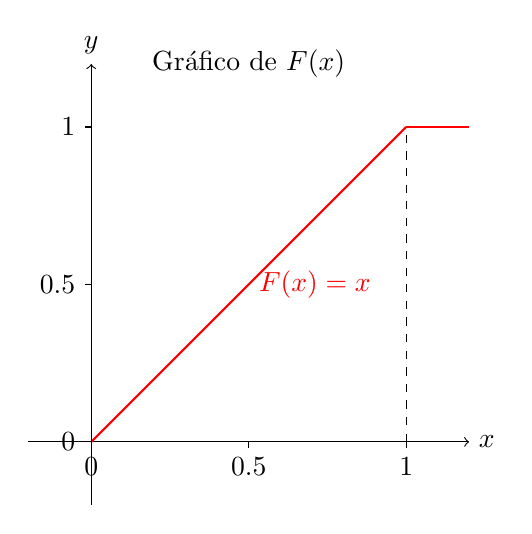
\begin{tikzpicture}[scale=4] % Escala de 4 cm por unidad
        % Ejes
        \draw[->] (-0.2,0) -- (1.2,0) node[right] {$x$};
        \draw[->] (0,-0.2) -- (0,1.2) node[above] {$y$};

        % Gráfico de F(x)
        \draw[red, thick] (0,0) -- (0,0); % Punto (0,0)
        \draw[red, thick] (0,0) -- (1,1) node[midway, right] {$F(x) = x$}; % Línea diagonal
        \draw[red, thick] (1,1) -- (1,1); % Punto (1,1)
        \draw[red, thick] (1,1) -- (1.2,1); % Línea horizontal en y=1

        % Trazar línea de referencia
        \draw[dashed] (0,0) -- (0,1);
        \draw[dashed] (1,0) -- (1,1);

        % Marcas en los ejes
        \foreach \x in {0, 0.5, 1} {
            \draw (\x,0) -- (\x,-0.02) node[below] {\x};
        }
        \foreach \y in {0, 0.5, 1} {
            \draw (0,\y) -- (-0.02,\y) node[left] {\y};
        }

        % Título
        \node at (0.5, 1.2) {Gráfico de $F(x)$};
    \end{tikzpicture}
\end{minipage}
\end{center}

El valor promedio de la distribución uniforme está dado por:

$$E(x) = \int_{0}^1 x \times f(x)dx$$

$$= \int_{0}^{1} x \times 1 \, {dx}$$

$$
= \left[ \frac{x^2}{2} \right]_{0}^{1}$$ 
$$ = \frac{1^2}{2} - \frac{0^2}{2} $$ 
$$= \frac{1}{2} $$

De igual manera se puede constatar que la varianza de la distribución está dada por (considerar $\mu = \frac{1}{n} \int_{i=1}^{n} x_i$):


$$\sigma^2 = \int_{0}^{1} (x-\mu)^2 * f(x) \, dx$$

$$\sigma^2 = \int_{0}^{1} (x-\frac{1}{2})^2 * 1 \, dx$$

$$\sigma^2 = \int_{0}^{1} x^2- \frac{2x}{2} + \frac{1}{4} \, dx$$

$$\sigma^2 = \int_{0}^{1} x^2- x+ \frac{1}{4} \, dx$$

$$
\sigma^2 = \int_{0}^{1} x^2 \, dx - \int_{0}^{1} x \, dx + \int_{0}^{1} \frac{1}{4} \, dx
$$

$$
\sigma^2 = \left[ \frac{x^3}{3} \right]_{0}^{1} - \left[ \frac{x^2}{2} \right]_{0}^{1} + \left[ \frac{x}{4} \right]_{0}^{1}
$$

$$
\sigma^2 = \frac{1}{3} - \frac{1}{2} + \frac{1}{4}
$$

$$\sigma^2 = \frac{1}{12}$$

La desviación estándar está dada por la raíz cuadrada de su varianza.

$$\sigma = \sqrt{\frac{1}{12}}$$

\section{Pruebas de Promedio}

Con la información anterior es posible entonces plantear una prueba de hipótesis de promedios, y una prueba de hipótesis de variancia. Con las cuales se trata de demostrar que los números pseudoaleatorios provienen de una distribución cuya media y variancia es igual a la distribución uniforme.


Para el planteamiento de la prueba de hipótesis se deben realizar los siguientes pasos:


\subsection{Formular la hipótesis nula y la hipótesis alternativa.}
$$H_0 = \mu = \frac{1}{2}$$
$$H_1 = \mu \not = \frac{1}{2}$$

\subsection{ Generar una muestra} 
Se generarán $n$ números aleatorios a los que llamaremos $x_1,x_2,\dots,x_n$ y obtener su promedio mediante la fórmula:

$$\bar{x} = \frac{\sum\limits_{i=1}^{n}x_i}{n}$$

\subsubsection{Determinar el valor de $z_0$}
$$z_0 = \frac{\bar{x}-\mu}{\sigma[\bar{x}]}$$

$$z_0  = \frac{\bar{x} - \mu}{\frac{\sigma}{\sqrt{n}}}$$

\subsection{Aceptación o rechazo de $z_0$}
Se compara el valor de $z_0$ con los valores que indican la zona de aceptación o rechazo en la función normal. Para encontrar estos valores se utiliza el valor predeterminado de $\alpha$ (ver figura \ref{fig:normalConfianza} de la página \pageref{fig:normalConfianza}.

\begin{figure}[ht]
    \centering
    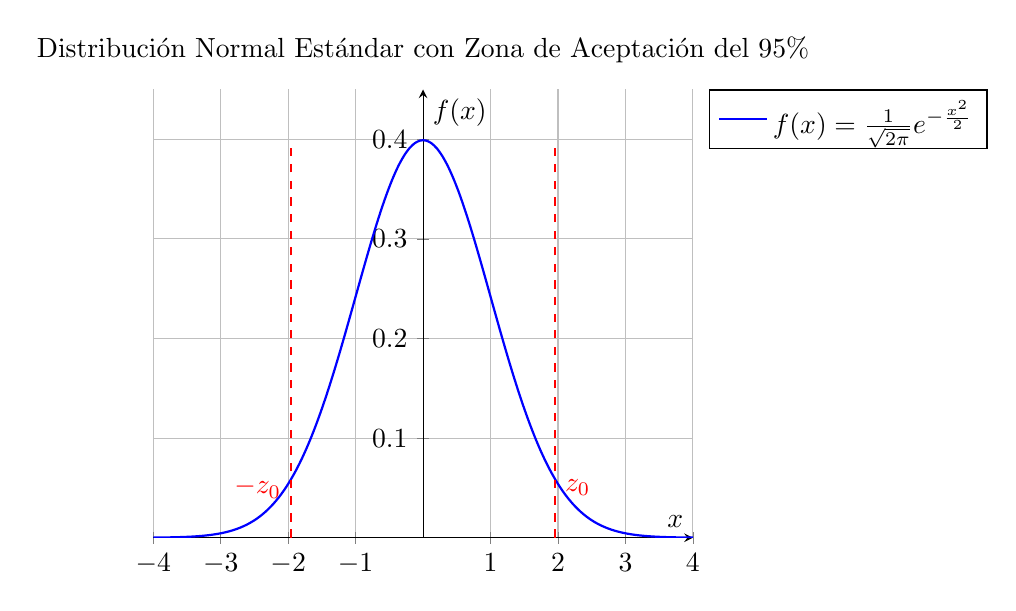
\begin{tikzpicture}
        \begin{axis}[
            axis lines=middle,
            xlabel={$x$},
            ylabel={$f(x)$},
            ymin=0, ymax=0.45,
            xmin=-4, xmax=4,
            xtick={-4,-3,-2,-1,0,1,2,3,4},
            ytick={0,0.1,0.2,0.3,0.4},
            domain=-4:4,
            samples=100,
            smooth,
            legend pos=outer north east,
            grid = both,
            title={Distribución Normal Estándar con Zona de Aceptación del 95\%}
        ]
        % Función de densidad de la normal
        \addplot[blue, thick] {1/sqrt(2*pi) * exp(-x^2/2)};
        \addlegendentry{$f(x) = \frac{1}{\sqrt{2\pi}} e^{-\frac{x^2}{2}}$}

        % Líneas de z_0 y -z_0
        \addplot[red, dashed, thick] coordinates {(-1.96, 0) (-1.96, 0.4)};
        \addplot[red, dashed, thick] coordinates {(1.96, 0) (1.96, 0.4)};
        
        % Etiquetas para las líneas de z_0
        \node at (axis cs:-1.96,0.05) [anchor=east, red] {$-z_0$};
        \node at (axis cs:1.96,0.05) [anchor=west, red] {$z_0$};
        
        \end{axis}
    \end{tikzpicture}
    \caption{Distribución normal estándar con $z_0$ para 95\%.}
    \label{fig:normalConfianza}
\end{figure}

\subsubsection{Ejemplo}
Se tienen los siguientes números aleatorios y se desea relizar una prueba de promedios para establecer si corresponden a un buen generador. Para ello se debe usar un valor de $\alpha =0.05$. A continuación se presentan los estadísticos que tienen los números generados.
\begin{verbatim}

----------------------------------------------
0.4237  0.2403  0.6000  0.7837  0.5281  0.4016
0.0290  0.8831  0.0337  0.8105  0.5314  0.9726
0.7655  0.7330  0.5237  0.0215  0.2666  0.9657
0.4849  0.2215  0.3961  0.9257  0.5494  0.3063
0.5863  0.0741  0.8169  0.8794  0.6554  0.0222
----------------------------------------------
\end{verbatim}

Se generan las hipótesis:

$$H_0 = \mu = \frac{1}{2}$$
$$H_1 = \mu \not = \frac{1}{2}$$



Se calculan los estadísticos:

$$n = 30$$
$$\bar{x} = 0.5144$$

Calculamos z0.

$$z_0 = \frac{\bar{x}-\mu}{\sigma[\bar{x}]}$$


$$z_0  = \frac{\bar{x} - \mu}{\frac{\sigma}{\sqrt{n}}}$$

$$z_0  = \frac{0.5144 - 0.5}{\frac{\sqrt{\frac{1}{12}}}{\sqrt{30}}}$$

$$z_0  = \frac{0.5144 - 0.5}{\frac{0.2887}{5.4772}}$$

$$z_0  = \frac{0.0144}{0.0527}$$

$$z_0  = 0.2732$$

Encontramos los valores de la zona de aceptación y rechazo. Cuando se tienen menos de 30 observaciones se suele usar la distribución de $t-student$, sin embargo para nuestro ejemplo se utilizará la distribución normal. Se tiene que el valor de $\alpha = 0.05$ por lo que la zona de aceptación de $H_O$ debe de tener un $0.95$ de la distribución, es decir, estar dentro del área de la figura \ref{fig:normalConfianza} en la página \pageref{fig:normalConfianza}, donde $-z_{\frac{\alpha}{2}} = -1.96$ y $z_{\frac{\alpha}{2}} = 1.96$.


Como $-1.96 \leq 0.2732 \leq 1.96$, se mantiene la hipótesis de $H_0$ y por lo tanto se concluye que los números generados provienen de una distribución cuya media es $0.5$.

\subsection{Forma alterna con un intervalo de confianza.}
 Una forma alterna como se puede realizar la parte final de la prueba es por medio de un intervalo de confianza. En este caso tenemos que:

 $$z(0.025)  =  \frac{(L - \mu)}{ o[\bar{x}]} $$

 $$z(0.025) \times  o[\bar{x}]  =  L - \mu$$

 $$\mu  +  z(0.025)*o[\bar{x}] = L$$

  $$L = \mu  +  z(0.025)*o[\bar{x}] $$

  $$L = \mu + z(0.025)*(\frac{o}{\sqrt{n}})$$

De esta forma se pueden obtener los límites para el valor promedio calculado mediante las fórmulas, el límite inferior se calcula con el valor negativo de zeta.

\[
L_{\text{inf}} = \mu - z(0.025) \cdot \left( \frac{o}{\sqrt{n}} \right)
\]

Sustituyendo los valores:

\[
L_{\text{inf}} = 0.50 - 1.96 \cdot \left( \frac{\sqrt{\frac{1}{12}}}{\sqrt{30}} \right)
\]

Calculando:

\[
L_{\text{inf}} = 0.50 - 1.96 \cdot 0.0527
\]

Finalmente:

\[
L_{\text{inf}} = 0.3967
\]

y el límite superior se puede calcular mediante con el límite positivo.

\[
L_{\text{sup}} = u + z(0.025) \cdot \left( \frac{o}{\sqrt{n}} \right)
\]

Sustituyendo los valores:

\[
L_{\text{sup}} = 0.50 + 1.96 \cdot \left( \frac{\sqrt{\frac{1}{12}}}{\sqrt{30}} \right)
\]

Calculando:

\[
L_{\text{sup}} = 0.50 + 1.96 \cdot 0.0527
\]

Finalmente:

\[
L_{\text{sup}} = 0.6033
\]

Si el valor de promedio de los datos se encuentra dentro del intervalo $[L_{inf}, L_{sup}]$ se acepta la hipótesis nula. En nuestro caso:

$$\bar{x} \in [L_{inf}, L_{sup}]$$ dado que $$0.5144  \in [0.3967 , 0.6033]$$

Y por lo tanto se acepta la hipótesis $H_0$.

\section{Prueba de Varianza}


Esta prueba consiste en verificar si los números aleatorios generados tienen una varianza de $\frac{1}{12}$ 
tal como la distribución uniforme.

\subsection{Formular $H_0$ y $H_1$}
$$H_0: o^2  = \frac{1}{12}$$

$$H_1: o^2  \not= \frac{1}{12}$$

\subsection{Muestreo}
Se genera una muestra de $n$ números aleatorios, a los que llamaremos $x_1, x_2, x_3, \dots, x_n$ y obtener su varianza mediante la fórmula:

\[
s^2 = \frac{1}{n-1} \sum_{i=1}^{n} (x_i - \bar{x})^2
\]

donde \( \bar{x} \) es la media de la muestra, dada por:

\[
\bar{x} = \frac{1}{n} \sum_{i=1}^{n} x_i
\]

\subsection{Determinar $\chi^2_0$}

$$\chi^2_0 = \frac{(n-1)\times s^2}{\sigma^2}$$

\subsection{Valorar confianza}
Se compara el valor de $\chi^2_0$ con los valores que indican la zona de aceptación o rechazo en la función $\chi^2$
Para encontrar estos valores se utiliza el valor predeterminado de $\alpha$.

\begin{center}
\begin{tikzpicture}{label=fig:chi}
\begin{axis}[
    axis lines=left,
    xlabel={$\chi^2$},
    ylabel={$f(\chi^2)$},
    domain=0:20,
    samples=200,
    ymin=0,
    ymax=0.5,
    xmin=0,
    xmax=20,
    width=12cm,
    height=8cm,
    ]
    
    % Para k=5: gamma(5/2) = 1.5*gamma(1.5) = 1.5*0.5*sqrt(pi) ≈ 1.329
    % Constante: 1/(2^2.5 * 1.329) ≈ 0.1766
    \addplot[thick, blue, name path=chi] {0.1766*x^(1.5)*exp(-x/2)};
    
    \path[name path=axis] (axis cs:0,0) -- (axis cs:20,0);
    
    \addplot[fill=red!30, opacity=0.5] fill between[
        of=chi and axis,
        soft clip={domain=0:1.145}
    ];
    
    \addplot[fill=red!30, opacity=0.5] fill between[
        of=chi and axis,
        soft clip={domain=12.833:20}
    ];
    
    \addplot[fill=green!20, opacity=0.5] fill between[
        of=chi and axis,
        soft clip={domain=1.145:12.833}
    ];
    
    \addplot[dashed, red, thick] coordinates {(1.145,0) (1.145,0.4)};
    \addplot[dashed, red, thick] coordinates {(12.833,0) (12.833,0.15)};
    
    \node[below] at (axis cs:1.145,0) {$\chi^2_{\alpha/2}$};
    \node[below] at (axis cs:12.833,0) {$\chi^2_{1-\alpha/2}$};
    \node at (axis cs:0.5,0.15) {$\alpha/2$};
    \node at (axis cs:16,0.08) {$\alpha/2$};
    \node at (axis cs:7,0.25) {$1-\alpha$};
    
\end{axis}
\end{tikzpicture}
\end{center}

\subsection{Ejemplo}
Se han generado 30 números aleatorios que se muestran a continuación y se desea relizar una prueba de varianza para establecer si corresponden a un buen generador. Para ello se debe usar un valor de $\alpha = 0.05$. A continuación se presentan los estadísticos que tienen los números generados.

\begin{verbatim}
----------------------------------------------
0.4237  0.2403  0.6000  0.7837  0.5281  0.4016
0.0290  0.8831  0.0337  0.8105  0.5314  0.9726
0.7655  0.7330  0.5237  0.0215  0.2666  0.9657
0.4849  0.2215  0.3961  0.9257  0.5494  0.3063
0.5863  0.0741  0.8169  0.8794  0.6554  0.0222
----------------------------------------------
\end{verbatim}
\subsubsection{Se generan hipótesis}
$$H_0: o^2  = \frac{1}{12}$$

$$H_1: o^2  \not= \frac{1}{12}$$

\subsubsection{Cálculo de estadígrafos}
$$n  = 30$$

$$\bar{x} = 0.5144$$

$$\epsilon^2  = 0.0930$$

\subsubsection{Calculamos $\chi^2_0$}

$$\chi^2_0 = \frac{(n-1) \times s^2}{\sigma^2}$$

$$\chi^2_0 = \frac{29 \times 0.093}{\frac{1}{12}}$$

$$\chi^2_0 = {29 \times 0.093 \times 12}$$

$$\chi^2_0 = 32.364$$

\subsubsection{Zona de aceptación}
Encontramos los valores de la zona de aceptación y rechazo. Se tiene que el valor de $\alpha = 0.05$ por lo que la zona de aceptación de $H_0$ debe de tener un $0.95$ de la distribución, por lo tanto se debe buscar en la distribución de $\chi^2$ con 29 grados de libertad, bajo las columnas de $0.025$ y $0.9750$.

\begin{center}
    \begin{tikzpicture}
\begin{axis}[
    axis lines=left,
    xlabel={$\chi^2$},
    ylabel={$f(\chi^2)$},
    domain=5:60,
    samples=300,
    ymin=0,
    xmin=0,
    xmax=65,
    width=14cm,
    height=8cm,
    title={Distribución $\chi^2$ con 29 grados de libertad, $\alpha=0.05$},
    ]
    
    % Función chi cuadrado con k=29 usando la forma simplificada
    % Para k grande, chi^2 se aproxima a una normal
    \addplot[thick, blue, name path=chi, samples=400] 
        {exp(-0.5*((x-29)/sqrt(2*29))^2)/(sqrt(2*pi*2*29))};
    
    % Línea base
    \path[name path=axis] (axis cs:0,0) -- (axis cs:65,0);
    
    % Región de rechazo izquierda (α/2 = 0.025)
    \addplot[fill=red!40, opacity=0.6] fill between[
        of=chi and axis,
        soft clip={domain=5:16.047}
    ];
    
    % Región de aceptación (0.95)
    \addplot[fill=green!30, opacity=0.6] fill between[
        of=chi and axis,
        soft clip={domain=16.047:45.722}
    ];
    
    % Región de rechazo derecha (α/2 = 0.025)
    \addplot[fill=red!40, opacity=0.6] fill between[
        of=chi and axis,
        soft clip={domain=45.722:60}
    ];
    
    % Líneas verticales para valores críticos
    \addplot[dashed, red, very thick] coordinates {(16.047,0) (16.047,0.05)};
    \addplot[dashed, red, very thick] coordinates {(45.722,0) (45.722,0.05)};
    
    % Etiquetas para valores críticos
    \node[below, align=center, font=\small] at (axis cs:16.047,0) 
        {$\chi^2_{0.025} = 16.047$};
    \node[below, align=center, font=\small] at (axis cs:45.722,0) 
        {$\chi^2_{0.975} = 45.722$};
    
    % Etiquetas para las regiones
    \node[red, font=\small] at (axis cs:10,0.04) {$\alpha/2=0.025$};
    \node[green!40!black, font=\small] at (axis cs:30,0.05) {$1-\alpha=0.95$};
    \node[red, font=\small] at (axis cs:52,0.04) {$\alpha/2=0.025$};
    
\end{axis}
\end{tikzpicture}
\end{center}

Los valores de los intervalos de confianza son : $16.0471$ y $45.7223$ (más exactamente de lo que se ve en el gráfico). Como $16.0471 \leq 32.3640 \leq 45.7223$, se mantiene la hipótesis de $H_0$ y por lo tanto se concluye que los números generados provienen de una distribución cuya varianza concuerda con la distribución uniforme.


\subsection{Intervalo de Confianza}

Al igual que antes también se pueden construir intervalos de confianza para el valor calculado de la varianza.

$$\chi^2_{\frac{\alpha}{2}} = \frac{(n-1)\times L}{\sigma^2}$$

$$\chi^2_{\frac{\alpha}{2}} = \frac{(n-1)\times L}{\frac{1}{12}}$$

$$\chi^2_{\frac{\alpha}{2}} = 12 \times (n-1) \times L$$

$$\frac{\chi^2_{\frac{\alpha}{2}}}{12 \times (n-1)} =  L$$

El límite inferior se calcula mediante la fórmula:

$$L_{inf} = \frac{\chi^2_{\frac{1-\alpha}{2}, n-1}}{12 \times (n-1)}$$

$$L_{inf} = \frac{16.0471}{12\times 29}$$

$$L_{inf} = 0.0461$$

El límite superior se calcula mediante la fórmula:

$$L_{sup} = \frac{\chi^2_{\frac{\alpha}{2}, n-1}}{12 \times (n-1)}$$

$$L_{sup} = \frac{45.7223}{12*29}$$

$$L_{sup} = 0.1314$$

Si varianza de los datos se encuentra dentro del intervalo $[L_{inf}, L_{sup}]$ se acepta la hipótesis nula. En nuestro caso:

$$s^2 \in [L_{inf}, L_{sup}]$$ dado que
$$0.0930 \in [0.0461 , 0.1314]$$

Y por lo tanto se acepta la hipótesis $H_0$.


\section{Prueba de corridas}
La prueba de las corridas busca estudiar el comportamiento de los números sucesivos generados. A continuación se esboza el proceso.

\subsection{Hipótesis del problema}
$$H_0: \text{Es una distribución uniforme}$$
$$H_1: \text{NO es una distribución uniforme}$$

\subsection{Clasificación de números}
Clasificar cada número aleatorio con respecto al anterior de acuerdo a la siguiente función:

$$
f(n_i,n_{i+1}) = \begin{cases}
+ & \text{si } n_i \leq n_{i+1} \\
- & \text{si } n_i > n_{i+1} 
\end{cases}
$$

\subsection{Cálculo de $h$}
Calcular el número de corridas, que denominaremos como $h$. Cada vez que cambia el signo se suma uno al número de corridas.

\subsection{Cálculo de esperanza y varianza de $h$}
Calcular esperanza y la variancia de $h$. Por medio de las fórmulas presentadas, en este caso $n$ representa el total de datos.
$$E(h) = \frac{2\times n -1}{3}$$

$$\sigma(h)^2 = \frac{16*n-29}{90}$$

$$\sigma(h) = \sqrt{\frac{16*n-29}{90}}$$

\subsection{Cálculo de $z_0$}
Se calcula el valor de $z_0$ y el valor del punto de rechazo denominado  $z_\frac{\alpha}{2}$. Si $z_0 \leq z_\frac{\alpha}{2} $ se acepta $H_0$.

$$z_0 = \frac{h-E(h)}{s(h)}$$

\subsection{Ejemplo}
A continuación se presenta un ejemplo. Suponga que se tienen los siguientes números producidos por un generador pseudoaleatorio. Se desea utilizar un nivel de $\alpha = 0.05$ para determinar si provienen o no de una distribución uniforme.
\begin{verbatim}
----------------------------------------------
0.4237  0.2403  0.6000  0.7837  0.5281  0.4016
0.0290  0.8831  0.0337  0.8105  0.5314  0.9726
0.7655  0.7330  0.5237  0.0215  0.2666  0.9657
0.4849  0.2215  0.3961  0.9257  0.5494  0.3063
0.5863  0.0741  0.8169  0.8794  0.6554  0.0222
----------------------------------------------
\end{verbatim}
A continuación se calculan las corridas para estos números, para el presente ejemplo se supone que los números fueron generados por columnas, puede constatarse que h = 22.


\begin{tabular}{lccc}
  & Valor & Símbolo & $h_i$ \\
$x_1$  & 0.4237 & $\dots$ & $\dots$ \\
$x_2$  & 0.0290 & $-$ & 1 \\
$x_3$  & 0.7655 & $+$ & 2 \\
$x_4$  & 0.4849 & $-$ & 3 \\
$x_5$ & 0.5863 & $+$ & 4 \\
$x_6$ & 0.2403 & $-$ & 5 \\
$x_7$ & 0.8831 & $+$ & 6 \\
$x_8$ & 0.7330 & $-$ & 7 \\
$x_9$  & 0.2215 & $-$ & 7 \\
$x_{10}$ & 0.0741 & $-$ & 7 \\
$x_{11}$ & 0.6000 & $+$ & 8 \\
$x_{12}$ & 0.0337 & $-$ & 9 \\
$x_{13}$ & 0.5237 & $+$ & 10 \\
$x_{14}$ & 0.3961 & $-$ & 11 \\
$x_{15}$ & 0.8169 & $+$ & 12 \\
$x_{16}$ & 0.7837 & $-$ & 13 \\
$x_{17}$ & 0.8105 & $+$ & 14 \\
$x_{18}$ & 0.0215 & $-$ & 15 \\
$x_{19}$ & 0.9257 & $+$ & 16 \\
$x_{20}$ & 0.8794 & $-$ & 17 \\
$x_{21}$ & 0.5281 & $-$ & 17 \\
$x_{22}$ & 0.5314 & $+$ & 18 \\
$x_{23}$ & 0.2666 & $-$ & 19 \\
$x_{24}$ & 0.5494 & $+$ & 20 \\
$x_{25}$ & 0.6554 & $+$ & 20 \\
$x_{26}$ & 0.4016 & $-$ & 21 \\
$x_{27}$ & 0.9726 & $+$ & 22 \\
$x_{28}$ & 0.9657 & $-$ & 23 \\
$x_{29}$ & 0.3063 & $-$ & 23 \\
$x_{30}$ & 0.0222 & $-$ & 23 \\\hline
\end{tabular}

\subsubsection{Cálculo de $E(h)$ y $\sigma(h)$}
$$E(h) = \frac{(2n-1)}{3}$$

$$E(h) = \frac{(2(30)-1)}{3}$$

$$E(h) = 19.6666$$

$$\sigma(h) = \sqrt{\frac{16n-29}{90}}$$

$$\sigma(h) = \sqrt{\frac{16(30)-29}{90}}$$
$$\sigma(h) = \sqrt{\frac{451}{90}}$$
$$\sigma(h) = \sqrt{5.0111}$$
$$\sigma(h) = 2.2386$$

\subsubsection{Cálculo de $z_0$}

$$z_0 = \frac{h-E(h)}{\sigma(h)}$$

$$z_0 = \frac{23-19.6666}{2.2386}$$
$$z_0   = 1.4890$$

Finalmente se calcula el valor del punto de rechazo, para un valor de $\alpha = 0.05$ en una tabla normal.

$$Z_{\frac{1-\alpha}{2}} = -1.96$$
$$Z_{\frac{\alpha}{2}}   = 1.96$$

Como  $-1.96 \leq 1.4890 \leq 1.96$, se mantiene la hipótesis de $H_0$ y por lo tanto se supone que los números provienen de una distribución uniforme.

\section{Pruebas de huecos con Dígitos}
Para este experimento estadístico se considera que todos los números aleatorios se encuentran unidos y se consideran una gran lista de dígitos. 

\subsection{Definición de $hueco$}

La prueba consiste en contar el número de dígitos diferentes que aparecen entre dos ocurrencias sucesivas de un mismo dígito. Por ejemplo si se tiene la cadena de números:

$$3178431133$$


Y estamos contando los $huecos$ que hay en el número tres (3), se tiene que de la primera aparición a la segunda hay un $hueco$ de tamaño $4$, de la segunda aparición a la tercera hay un $hueco$ de tamaño $2$ y de la tercera aparición a la cuarta hay un $hueco$ de tamaño $0$.

\subsection{Ejemplo de prueba}

Suponga que se tiene la siguiente secuencia de números aleatorios y se formará una lista de dígitos a partir de sus \textbf{columnas}, es decir se recorrerán los números de forma vertical. Asímismo al momento de formar los dígitos se toman en cuenta únicamente los que se encuentran después del punto decimal.

\begin{verbatim}
----------------------------------------------
0.4237  0.2403  0.6000  0.7837  0.5281  0.4016
0.0290  0.8831  0.0337  0.8105  0.5314  0.9726
0.7655  0.7330  0.5237  0.0215  0.2666  0.9657
0.4849  0.2215  0.3961  0.9257  0.5494  0.3063
0.5863  0.0741  0.8169  0.8794  0.6554  0.0222
----------------------------------------------

\end{verbatim}
\subsubsection{Contando $huecos$}
Si se realiza el conteo de huecos para cada uno de los dígitos se obtiene la siguiente tabla.

\begin{tabular}{c|cccccccccc|c}

{\textbf{$Hueco$}} & \multicolumn{10}{c|}{\textbf{Dígitos}} & {\textbf{Total}} \\\hline
& \textbf{0} & \textbf{1} & \textbf{2} & \textbf{3} & \textbf{4} & \textbf{5} & \textbf{6} & \textbf{7} & \textbf{8} & \textbf{9} & \\\hline

0  & 3 & 0 & 3 & 2 & 1 & 2 & 2 & 0 & 1 & 0 & 14 \\
1  & 1 & 1 & 0 & 1 & 2 & 0 & 1 & 1 & 0 & 0 & 7 \\
2  & 2 & 1 & 0 & 3 & 0 & 1 & 0 & 1 & 1 & 0 & 9 \\
3  & 0 & 0 & 2 & 2 & 1 & 2 & 2 & 1 & 1 & 1 & 12 \\
4  & 2 & 2 & 0 & 0 & 0 & 2 & 2 & 1 & 1 & 0 & 10 \\
5  & 0 & 0 & 0 & 0 & 1 & 1 & 0 & 1 & 1 & 2 & 6 \\
6  & 0 & 1 & 1 & 0 & 1 & 0 & 1 & 0 & 1 & 0 & 5 \\
7  & 0 & 1 & 1 & 0 & 1 & 1 & 0 & 0 & 0 & 0 & 4 \\
8  & 1 & 0 & 0 & 0 & 0 & 0 & 1 & 2 & 0 & 1 & 5 \\
9  & 0 & 0 & 0 & 1 & 0 & 0 & 0 & 1 & 0 & 1 & 3 \\
10 & 0 & 0 & 1 & 0 & 0 & 0 & 0 & 0 & 0 & 0 & 1 \\
11 & 1 & 0 & 1 & 0 & 1 & 1 & 0 & 1 & 1 & 0 & 6 \\
12 & 0 & 1 & 0 & 0 & 0 & 1 & 0 & 0 & 0 & 1 & 3 \\
13 & 0 & 0 & 0 & 0 & 0 & 0 & 1 & 0 & 0 & 0 & 1 \\
14 & 1 & 0 & 1 & 1 & 0 & 0 & 0 & 0 & 0 & 0 & 3 \\
15 & 0 & 2 & 1 & 0 & 0 & 0 & 0 & 0 & 0 & 1 & 4 \\
16 & 0 & 0 & 0 & 1 & 1 & 0 & 0 & 0 & 0 & 0 & 2 \\
17 & 0 & 0 & 1 & 0 & 0 & 0 & 0 & 0 & 0 & 0 & 1 \\
18 & 0 & 0 & 0 & 0 & 0 & 2 & 0 & 0 & 0 & 0 & 2 \\
19 & 0 & 0 & 1 & 0 & 0 & 0 & 0 & 1 & 0 & 0 & 2 \\
20 & 0 & 0 & 0 & 0 & 0 & 0 & 0 & 0 & 0 & 0 & 0 \\\hline

\textbf{Total} & \textbf{11} & \textbf{9} & \textbf{13} & \textbf{11} & \textbf{9} & \textbf{13} & \textbf{10} & \textbf{10} & \textbf{7} & \textbf{7} & \textbf{100} \\

\end{tabular}

Además de estos huecos se encontraron los siguientes huecos que no aparecen en la tabla:

\begin{enumerate}
\item Para el dígito 0, un hueco de tamaño 21.
\item Para el dígito 0, un hueco de tamaño 32

\item Para el dígito 3, un hueco de tamaño 22.
\item Para el dígito 3, un hueco de tamaño 26.

\item Para el dígito 4, un hueco de tamaño 40.

\item Para el dígito 6, un hueco de tamaño 21.
\item Para el dígito 6, un hueco de tamaño 30.

\item Para el dígito 7, un hueco de tamaño 27.

\item Para el dígito 8, un hueco de tamaño 30.

\item Para el dígito 9, un hueco de tamaño 37.
\end{enumerate}


Con estos 10 huecos adicionales se obtiene un total de 100 + 10 = 110 huecos en total. Con base en estos valores es que se construirán las frecuencias observadas de la tabla.

\subsection{Probabilidades de cada $hueco$}

Para construir las frecuencias esperadas, se deben establecer las probabilidades para cada tamaño de hueco. Es decir la probabilidad de que ocurra un hueco de tamaño $x$. Las cuales estarán dadas por:

$$P(x) = \frac{1}{10} \times (\frac{9}{10})^{x}$$
$$P(x) = 0.1 \times 0.9^{x}$$

Lo huecos pueden ser teóricamente de tamaño infinito, por lo cual en algún momento se tendrán que agrupar las probabilidades restantes. Para un hueco de tamaño mayor que n se tendría que:

$$P(x\geq n) = \sum_{i=n}^\infty (0.1)\times (0.9)^i$$

Factorizando:
$$P(x\geq n) = 0.1 \sum_{i=n}^\infty (0.9)^i$$

Usando la fórmula de serie geométrica $\displaystyle\sum_{i=k}^\infty r^i = \frac{r^k}{1-r}$ con $r=0.9$:

$$P(x\geq n) = 0.1 \cdot \frac{(0.9)^n}{1-0.9} = 0.1 \cdot \frac{(0.9)^n}{0.1} = (0.9)^n$$

$$P(x\geq n) = \left(\frac{9}{10}\right)^n = 0.9^n$$



Con base en las fórmulas anteriores, podemos calcular los valores de las probabilidades esperadas:

$$P(x=0) = 0.1\times 0.9^0 = 0.1000$$
$$P(x=1) = 0.1\times 0.9^1 = 0.0900$$
$$P(x=2) = 0.1\times 0.9^2 = 0.0810$$
$$P(x=3) = 0.1\times 0.9^3 = 0.0729$$
$$P(x=4) = 0.1\times 0.9^4 = 0.0656$$
$$P(x=5) = 0.1\times 0.9^5 = 0.0590$$
$$P(x=6) = 0.1\times 0.9^6 = 0.0531$$
$$P(x\geq 7) =  0.9^7 = 0.4783$$

\subsection{Tabla de valores esperados y observados}
Con base en los valores anteriores construimos una tabla que nos servirá para calcular el valor del estadístico de $\chi^2$.
\begin{verbatim}
    -------------------------------------------------------------------
                                                              2
                                                  2    (fo-fe)
 Huecos  fo     pe        fe      (fo-fe)   (fo-fe)    -------
                                                         fe
-------------------------------------------------------------------

   0     14    0.1000   11.0000    3.0000    9.0000    0.8182
   1      7    0.0900    9.9000   -2.9000    8.4100    0.8495
   2      9    0.0810    8.9100    0.0900    0.0081    0.0009
   3     12    0.0729    8.0190    3.9810   15.8484    1.9764
   4     10    0.0656    7.2160    2.7829    7.7445    1.0731
   5      6    0.0590    6.4954   -0.4954    0.2454    0.0378
   6      5    0.0531    5.8459   -0.8459    0.7155    0.1224
>= 7      4    0.4783   52.6127   -5.6127   31.5019    0.5988
-------------------------------------------------------------------
Total   110                                                       2
                                                                \/
                                                       5.4769 = /\
                                                                  0
-------------------------------------------------------------------

\end{verbatim}

Ahora, que tenemos el valor de $\chi^2_0$, tenemos que calcular el valor del punto de rechazo. Para esto se usa un valor de $\alpha =  0.05$ con $10-1=9$ grados de libertad.

$$\chi^2_{0.05,9} = 16.9190$$
Como el valor de $5.4769 \leq 16.9190$, se acepta $H_0$ y por lo tanto se supone que los números generados si corresponden a una distribución uniforme.


\section{Prueba de Huecos con Números}
Esta prueba de los huecos es bastante similar a la anterior, con la excepción que se toman los números pseudoaleatorios de forma independiente. A continuación se muestra el procedimiento

\subsection{Selección de intervalo}
Se debe seleccionar un intervalo $[inf,sup]$ dentro de $[0,1]$, es decir debe cumplir con las condiciones $0 \leq inf \leq sup \leq 1$.

\subsection{Definición de $hueco$}
Sea $N_j \in  [inf,sup]$  y de $N_{j+1},N_{j+2}, \dots, N_{j+i} \not \in [inf,sup]$ y $N_{j+i+1} \in [inf,sup]$ entonces se tiene un hueco de tamaño $i$.

\subsubsection{Ejemplo}
Supongamos $inf=0.3$ y $sup=0.7$ y que la siguiente sucesión de números pseudoaleatorios: $0.3251, 0.2224, 0.2114, 0.8810, 0.4733$ se tiene entonces un hueco de tamaño 3 ya que:

$$N_{j}   = 0.3251  \in [0.3,0.7]$$
$$N_{j+1} = 0.2224  \not \in [0.3,0.7]$$
$$N_{j+2} = 0.2114  \not \in [0.3,0.7]$$
$$N_{j+3} = 0.8810  \not \in [0.3,0.7]$$
$$N_{j+4} = 0.4733  \in [0.3,0.7]$$

Por lo tanto el hueco va desde $N_{j+1}$ hasta $N_{j+3}$ y es de tamaño $3$.

\subsection{Cálculo de probabilidad para el $hueco$}
Se calcula la distribución de probabilidad para el tamaño de cada hueco, la cual está dada por el área correspondiente a la distribución uniforme $t$, siendo $t = sup-inf$:

$$P(x) = t\times (1-t)^x$$

\subsection{Cálculo de estadísticos de $\chi^2$}
Finalmente se calculan los estadísticos de $\chi^2_0$ y los límites de confianza.

\subsection{Ejemplo}
A continuación presentamos un ejemplo. Supongamos que se tiene la siguiente muestra de números aleatorios.
\begin{verbatim}

------------------------------------------
0.3759   0.8998   0.9093   0.7532   0.1818
0.1978   0.1737   0.1437   0.6702   0.4732
0.0864   0.3891   0.4334   0.6318   0.4102
0.7861   0.7041   0.2486   0.1772   0.6703
0.2286   0.7594   0.2736   0.8711   0.9019
0.4140   0.0933   0.5509   0.0214   0.3632
0.6918   0.9706   0.9093   0.0402   0.9361
0.3934   0.2913   0.0289   0.2729   0.2577
0.1483   0.1439   0.3620   0.6796   0.5624
0.3116   0.2645   0.6868   0.5978   0.0785

0.2002   0.9430   0.2192   0.8039   0.1904
0.8411   0.2139   0.0094   0.1847   0.9256
0.3876   0.9332   0.8836   0.9821   0.7089
0.0133   0.5280   0.5559   0.8072   0.7755
0.7476   0.0165   0.5087   0.5476   0.0742
0.2152   0.5016   0.7021   0.8322   0.8921
0.7750   0.2476   0.5130   0.2951   0.3042
0.2346   0.5459   0.8465   0.3191   0.7506
0.5631   0.1351   0.9502   0.0233   0.0491
0.6755   0.2889   0.1925   0.5978   0.5320
------------------------------------------
\end{verbatim}

Se ha construido la siguiente tabla de frecuencias observadas. Para ello se utilizó un valor de $[inf,sup] = [0.3,0.7]$ y se encontraron los siguientes huecos.\\
\begin{center}
    
\begin{tabular}{|c|c|}
        \hline
        \textbf{Tamaño} & \textbf{$fo$} \\
        \textbf{Hueco} &\\ \hline
        0 & 9 \\ \hline
        1 & 8 \\ \hline
        2 & 6 \\ \hline
        $\geq 3$ & 9 \\ \hline
        \textbf{Total} & 32 \\ \hline
\end{tabular}\\

\end{center}
Con los valores utilizados, utilizando la distribución geométrica, con los valores utilizados se convierte en:


$$p(x)  =  0.4 (1 - 0.4)^x$$

$$p(x)  =  0.4 (0.6)^x$$


Con base en las fórmulas anteriores, podemos calcular los valores de las probabilidades esperadas.


$$p(x = 0)  =  0.4 (0.6)^0   =  0.4000$$

$$p(x = 1)  =  0.4 (0.6)^1   =  0.2400$$

$$p(x = 2)  =  0.4 (0.6)^2   =  0.1440$$

$$p(x>= 3)  =      (0.6)^3   =  0.2160$$

Podemos construir ahora la tabla para el cálculo de ji cuadrado.
\begin{verbatim}
    
------------------------------------------------------------------
                                                            2
                                                 2    (fo-fe)
Huecos  fo     pe        fe      (fo-fe)   (fo-fe)    -------
                                                        fe
------------------------------------------------------------------
   0     9    0.4000   12.8000   -3.8000   14.4400    1.1281
   1     7    0.2400    7.6800   -0.6800    0.4624    0.0602
   2     7    0.1440    4.6080    2.3920    5.7217    1.2417
 >=3     9    0.2160    6.9120    2.0880    4.3597    0.6308
------------------------------------------------------------------
Total   32                                                       2
                                                               \/
                                                      3.0608 = /\
                                                                 0
------------------------------------------------------------------
\end{verbatim}

Después de calcular el valor de $\chi^2_0$, tenemos que calcular el valor del punto de rechazo. Para esto se usa un valor de $\alpha = 0.05$ con $4-1=3$ grados de libertad.

$$\chi^2_{(0.05,3)} = 7.8147$$

Como el valor de $3.0608 \leq 7.8147$, se acepta $H_0$ y por lo tanto se supone que los números generados corresponden a una distribución uniforme.

\section{Prueba de Poker}
En esta prueba se tratan de trasladar las probabilidades del juego de naipes conocido como \textit{Póker}, a los números pseudoaleatorios generados. 

Como el juego de cartas se juega con 5 cartas se utilizarán números pseudoaleatorios de longitud 5, en caso que sean más largos se toman los primeros cinco números.\footnote{¿Análogamente a la prueba de huecos se pueden concatener todos los números y tomar quíntuplas de dígitos?} Se supondrá entonces que se juega con una baraja que tiene naipes que van del 0 al 9. Bajo estas condiciones se tienen los siguientes posibles resultados.

\begin{itemize}
    \item Todos los números son diferentes.
\item Un par, hay dos números iguales.
\item Dos pares, hay dos pares de números iguales.
\item Una tercia, tres números iguales.
\item Full House, una tercia y un par.
\item Póker, 4 números iguales.
\item Quintilla, 5 números iguales.
\end{itemize}

La quintilla existe únicamente para los números pseudoaleatorios pues en un juego de naipes no pueden existir cinco números iguales, a menos claro que alguien haga trampa \smiley.

\subsubsection{Ejemplo}
A continuación se presentan algunos ejemplos de como se deben clasificar los números.

\begin{itemize}
    \item 0.78961   todos diferentes
\item 0.76086   un par
\item 0.80548   un par
\item 0.58518   dos pares
\item 0.33317   una tercia
\item 0.89898   full house
\item 0.99990   póker
\item 0.55555   quintilla
\end{itemize}

A continuación se presenta una lista de 30 números con los cuales se realizará la prueba del póker.

\begin{verbatim}

----------------------------------------------------
0.72484  0.48999  0.50502  0.39528  0.36782  0.90234
0.71890  0.61234  0.86322  0.94134  0.99872  0.27657
0.34565  0.02345  0.67347  0.10987  0.25678  0.25593
0.82345  0.12387  0.05389  0.82472  0.59289  0.36782
0.03991  0.10461  0.93719  0.16894  0.98953  0.73231
----------------------------------------------------

\end{verbatim}

Al clasificar estos treinta números, se obtiene el siguiente resultado.

\begin{center}
 \begin{tabular}{|lc|}
        \hline
        \textbf{Clase} & \textbf{fo} \\ \hline\hline
        Diferentes & 13 \\ 
        Un par & 15 \\ 
        Dos pares & 1 \\ 
        Tercia & 1 \\ 
        Full & 0 \\ 
        Póker & 0 \\ 
        Quintilla & 0 \\ \hline
    \end{tabular}
\end{center}


Para calcular las frecuencias esperadas, debemos calcular inicialmente la probabilidad de cada posible ocurrencia. Observe que si se desean formar números con 5 dígitos decimales existen $100.000$ posibles números que van desde el $0.00000$ hasta el $0.99999$.
{
\begin{itemize}

\item $P(\text{diferentes}) = \frac{10\times 9 \times 8 \times 7\times 6}{10^5}\times \binom{5}{0} = 0.30240$

\item $P(\text{un par}) = \frac{10\times 1 \times 9 \times 8\times 7}{10^5} \times \binom{5}{2}= 0.50400$

\item $P(\text{dos pares}) = \frac{1}{2}\times \frac{10\times 1 \times 9 \times 1\times 8}{10^5} \times \binom{5}{2}\times \binom{3}{2}= 0.10800$


\item $P(\text{tercia}) = \frac{10\times 1 \times 1 \times 9\times 8}{10^5} \times \binom{5}{3}= 0.07200$

\item $P(\text{full house}) = \frac{10\times 1 \times 1 \times 9\times 1}{10^5} \times \binom{5}{3}\times \binom{2}{2}= 0.00900$

\item $P(\text{poker}) =  \frac{10\times 1 \times 1 \times 1\times 9}{10^5} \times \binom{5}{4} = 0.00450$

\item $P(\text{quintilla}) =  \frac{10\times 1 \times 1 \times 1\times 1}{10^5} \times \binom{5}{5} = 0.00010$


\end{itemize}
}


De esta forma tenemos que:

\begin{center}
    \begin{tabular}{lrl}
       p(diferentes)&=&0.3024 \\
p(un par)    &=&0.5040\\
p(dos pares) &=&0.1080\\
p(tercia)    &=&0.0720\\
p(full)      &=&0.0090\\
p(póker)     &=&0.0045\\
p(quintilla) &=&0.0001
    \end{tabular}
\end{center}

Con estas probabilidades esperadas se pueden calcular las frecuencias esperadas para realizar el cálculo de ji cuadrado.

\begin{verbatim}

------------------------------------------------------------------
                                                             2
                                                   2  (fo-fe)
 Clase       fo    pe       fe     (fo-fe)  (fo-fe)   -------
                                                        fe
------------------------------------------------------------------
Diferentes   13   0.3024   9.0720   3.9280  15.4292   1.7007
Un par       15   0.5040  15.1200  -0.1200   0.0144   0.0010
Dos pares     1   0.1080   3.2400  -2.2400   5.0176   1.5486
Tercia        1   0.0720   2.1600  -1.1600   1.3456   0.6230
Full          0   0.0090   0.2700  -0.2700   0.0729   0.2700
Póker         0   0.0045   0.1350  -0.1350   0.0182   0.1350
Quintilla     0   0.0001   0.0030  -0.0030   0.0000   0.0030
------------------------------------------------------------------
Total        30                                                  2
                                                               \/
                                                      4.2813 = /\
                                                                 0
------------------------------------------------------------------

\end{verbatim}

Para calcular el punto de rechazo utilizaremos un valor de $\alpha = 0.05$. Además de $7-1 = 6$ grados de libertad.


$$\chi^2_{(0.05,6)} = 12.5916$$

Como el valor de $4.2813 \leq 12.5916$, se acepta $H_0$ y por lo tanto se supone que los números generados corresponden a una distribución uniforme.




\section{Prueba de Series}


La prueba de series trata de evaluar el grado de aleatoriedad que existe entre números sucesivos. Lo que se hace es unir los números de dos en dos para formar puntos en un cuadrado de área $1$. 

\subsection{Emparejamiento}
Dado un conjunto de k números aleatorios se forman parejas tomando los números $n_i$ y $n_{i+1}$. Por ejemplo si se tienen 10 números aleatorios las parejas que se forman son:\\
\begin{itemize}
    \item[] $n_1$ con $n_2$
\item[] $n_2$ con $n_3$
\item[] $n_3$ con $n_4$
\item[] $n_4$ con $n_5$
\item[] $n_5$ con $n_6$
\item[] $n_6$ con $n_7$
\item[] $n_7$ con $n_8$
\item[] $n_8$ con $n_9$
\item[] $n_9$ con $n_{10}$
\end{itemize}

\subsection{Creando cuadrícula}
Luego se toma un cuadrado de área uno y se subdivide en secciones de igual tamaño. Supongamos que se construyen $c$ celdas en el eje $x$ y $c$ celdas en el eje $y$.

Luego, se determina la celda a la que pertenece cada pareja y se contabilizan las frecuencias observadas.

\subsection{Frecuencia esperada}
La frecuencia esperada ($fe$) está dada por una distribución uniforme de las parejas dentro de las celdas. A continuación se muestra la fórmula donde n representa el total de números aleatorios y c el número de celdas en un eje. Considerar que son $n-1$ pares o posiciones $(x,y)$
$$fe = \frac{n-1}{c^2}$$

\subsection{Ejemplo}
Por ejemplo, suponga que se tiene el siguiente conjunto compuesto por 100 números aleatorios.

\begin{verbatim}
------------------------------------------
0.3759   0.8998   0.9093   0.7532   0.1818
0.1978   0.1737   0.1437   0.6702   0.4732
0.0864   0.3891   0.4334   0.6318   0.4102
0.7861   0.7041   0.2486   0.1772   0.6703
0.2286   0.7594   0.2736   0.8711   0.9019
0.4140   0.0933   0.5509   0.0214   0.3632
0.6918   0.9706   0.9093   0.0402   0.9361
0.3934   0.2913   0.0289   0.2729   0.2577
0.1483   0.1439   0.3620   0.6796   0.5624
0.3116   0.2645   0.6868   0.5978   0.0785

0.2002   0.9430   0.2192   0.8039   0.1904
0.8411   0.2139   0.0094   0.1847   0.9256
0.3876   0.9332   0.8836   0.9821   0.7089
0.0133   0.5280   0.5559   0.8072   0.7755
0.7476   0.0165   0.5087   0.5476   0.0742
0.2152   0.5016   0.7021   0.8322   0.8921
0.7750   0.2476   0.5130   0.2951   0.3042
0.2346   0.5459   0.8465   0.3191   0.7506
0.5631   0.1351   0.9502   0.0233   0.0491
0.6755   0.2889   0.1925   0.5978   0.5320
------------------------------------------
\end{verbatim}


Tomando cada una de las 99 posibles parejas obtenemos las frecuencias observadas.
\begin{center}
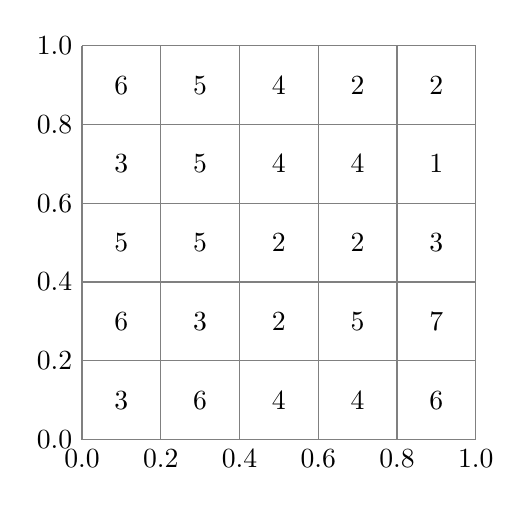
\begin{tikzpicture}[scale=5]
    % Dibujar la cuadrícula
    \draw[step=0.2, gray] (0,0) grid (1,1);
    
    % Etiquetas eje X
    \foreach \x in {0.0,0.2,0.4,0.6,0.8,1.0}
        \draw (\x,0) node[below] {\x};
    
    % Etiquetas eje Y
    \foreach \y in {0.0,0.2,0.4,0.6,0.8,1.0}
        \draw (0,\y) node[left] {\y};
    
    % Números en las celdas (fila por fila, de abajo hacia arriba)
    % Fila 0.0-0.2
    \node at (0.1,0.1) {3};
    \node at (0.3,0.1) {6};
    \node at (0.5,0.1) {4};
    \node at (0.7,0.1) {4};
    \node at (0.9,0.1) {6};
    
    % Fila 0.2-0.4
    \node at (0.1,0.3) {6};
    \node at (0.3,0.3) {3};
    \node at (0.5,0.3) {2};
    \node at (0.7,0.3) {5};
    \node at (0.9,0.3) {7};
    
    % Fila 0.4-0.6
    \node at (0.1,0.5) {5};
    \node at (0.3,0.5) {5};
    \node at (0.5,0.5) {2};
    \node at (0.7,0.5) {2};
    \node at (0.9,0.5) {3};
    
    % Fila 0.6-0.8
    \node at (0.1,0.7) {3};
    \node at (0.3,0.7) {5};
    \node at (0.5,0.7) {4};
    \node at (0.7,0.7) {4};
    \node at (0.9,0.7) {1};
    
    % Fila 0.8-1.0
    \node at (0.1,0.9) {6};
    \node at (0.3,0.9) {5};
    \node at (0.5,0.9) {4};
    \node at (0.7,0.9) {2};
    \node at (0.9,0.9) {2};
\end{tikzpicture}
\end{center}

Las frecuencias esperadas están dadas al distribuir las 99 parejas de manera uniforme sobre el cuadriculado. Esto es equivalente a dividir 99 entre las 25 casillas que existen.

$$fe = \frac{n-1}{c^2} = \frac{100-1}{5^2} =\frac{99}{25} = 3.9600$$


Ahora con las frecuencias observadas y las frecuencias esperadas se construye las estimaciones de $\chi^2$.

\begin{verbatim}
--------------------------------------------------------
                                                 2
                                      2   (fo-fe)
 Celda   fo     fe    (fo-fe)   (fo-fe)   -------
                                            fe
--------------------------------------------------------
   1      6    3.96    2.0400    4.1616    1.0509
   2      5    3.96    1.0400    1.0816    0.2731
   3      4    3.96    0.0400    0.0016    0.0004
   4      2    3.96   -1.9600    3.8416    0.9701
   5      2    3.96   -1.9600    3.8416    0.9701
   6      3    3.96   -0.9600    0.9216    0.2327
   7      5    3.96    1.0400    1.0816    0.2731
   8      4    3.96    0.0400    0.0016    0.0004
   9      4    3.96    0.0400    0.0016    0.0004
  10      1    3.96   -2.9600    8.7616    2.2125
  11      5    3.96    1.0400    1.0816    0.2731
  12      5    3.96    1.0400    1.0816    0.2731
  13      2    3.96   -1.9600    3.8416    0.9701
  14      2    3.96   -1.9600    3.8416    0.9701
  15      3    3.96   -0.9600    0.9216    0.2327
  16      6    3.96    2.0400    4.1616    1.0509
  17      3    3.96   -0.9600    0.9216    0.2327
  18      2    3.96   -1.9600    3.8416    0.9701
  19      5    3.96    1.0400    1.0816    0.2731
  20      7    3.96    3.0400    9.2416    2.3337
  21      3    3.96   -0.9600    0.9216    0.2327
  22      6    3.96    2.0400    4.1616    1.0509
  23      4    3.96    0.0400    0.0016    0.0004
  24      4    3.96    0.0400    0.0016    0.0004
  25      6    3.96    2.0400    4.1616    1.0509
--------------------------------------------------------
Total    99                                            2
                                                     \/
                                          15.8990  = /\
                                                       0
--------------------------------------------------------
\end{verbatim}


Después de calcular el valor de $\chi^2_0$, tenemos que calcular el valor del punto de rechazo. Para esto se usa un valor de $\alpha$ de 0.05 con 25-1=24 grados de libertad.

$$\chi^2_{0.05,24} = 36,415$$


Como el valor de $15.8990 \leq 36.4150$, se acepta $H_0$ y por lo tanto se supone que los números generados corresponden a una distribución uniforme.

\section{Resumen}

Se han presentado múltiples pruebas para corroborar que un conjunto de números pseudoaleatorios correspondan efectivamente a una distribución de probabilidad uniforme.

Una sola prueba no basta para demostrar que un conjunto de números cumplen con las condiciones solicitadas, sin embargo un conjunto de números que efectivamente hayan sido generados por una distribución uniforme debe cumplir positivamente con todas las pruebas descritas.

Finalmente es importante destacar que una vez que se han presentado estos ejemplos de pruebas debe ser relativamente sencillo modificar o combinar las pruebas para producir otra prueba nueva y original.



\section{Ejercicios}

\begin{enumerate}


\item Para techar un estadio se ha concedido el contrato a la compañía WestGate y asociados. Las especificaciones del edificio exigen un techo móvil cubierto por 10000 láminas de aluminio de 0.04 pulgadas de espesor. Las láminas no pueden ser más gruesas por la resistencia del techo, ni más delgadas por durabilidad.

Por esa razón se examinarán las láminas del proveedor. Para ello se toma una muestra de 100 láminas de manera aleatoria. Estas presentaron un espesor de 0.0408 pulgadas, con una desviación estándar de 0.004 pulgadas.
\begin{enumerate}[label=\alph*.]
    \item Haga una prueba de hipótesis para determinar si las láminas cumplen o no con los requisitos. Utilice un nivel de $\alpha = 0.05$
    \item Establezca un intervalo de confianza que indique dentro de qué parámetros debió estar el promedio de la muestra para ser aceptado con 0.05
\end{enumerate}
\item Un profesor de computación ha reflexionado profundamente sobre el diseño de los exámenes. Para que tenga una seguridad razonable de que un examen logra distinguir bien las diferencias en el aprovechamiento logrado por los estudiantes, la desviación estándar de las notas de los exámenes no debe ser muy pequeña pues todos tendrían una nota cercana, de igual manera no debe ser muy grande pues habría una tendencia a notas demasiado bajas, lo que no favorece la moral de los alumnos. Su experiencia le hace pensar que una desviación estándar de 13 puntos en un examen de 100 puntos indica que el examen logra equilibrar debidamente los dos objetivos.

El profesor acaba de administrar un examen a un grupo de 31 alumnos, la puntuación promedio fue de 72.70 y la desviación estándar fue de 15.9 

Realice una prueba de hipótesis de varianzas para demostrar si el supuesto del profesor es correcto o no. Sugerencia, debe usar una hipótesis nula de $\sigma = 13$, o en su defecto que $\sigma^2 = 169$.



\item A continuación se presenta una tabla con 30 números pseudoaleatorios. Suponga que los números vienen en columnas, es decir procese la primera columna, luego la segunda y por último la tercera columna para realizar las pruebas que se le solicitan. Para todas las pruebas utilice un valor de $\alpha$ de 0.05

\begin{verbatim}

---------------------------------------------------
0.7595   0.8716   0.4833   0.1373   0.0348   0.4988
0.5679   0.4649   0.1820   0.2033   0.5024   0.2933
0.3826   0.2801   0.0192   0.3295   0.2756   0.7712
0.5569   0.3824   0.6657   0.8896   0.0532   0.3213
0.5449   0.2334   0.8826   0.6979   0.5891   0.8457
---------------------------------------------------
\end{verbatim}
\begin{enumerate}[label=\alph*.]
\item Realice una prueba de promedios.
\item  Realice una prueba de variancia.
\item  Realice una prueba de corridas.
\item  Realice una prueba de huecos con dígitos.
\item  Realice una prueba de huecos con números.
\item  Realice una prueba de póker.
\item  Realice una prueba de series.
\end{enumerate}


\item Para el siguiente conjunto de números realice una prueba de promedios y una prueba de varianza, para determinar si los números generados pertenecen o no a una distribución uniforme entre 0 y 9.

\begin{verbatim}
----------------------
3  0  9  1  7  6  1  0
0  1  4  0  2  0  2  3
1  3  2  3  0  5  1  8
7  9  5  5  9  4  2  0
6  0  4  1  7  8  9  8
----------------------    
\end{verbatim}




\item A continuación se presentan 30 números. Utilice una prueba de corridas para determinar si pertenecen a una distribución uniforme continua entre $[0,1]$.
\begin{verbatim}
---------------------------------------------------
0.2216   0.0338   0.4328   0.0552   0.4371   0.4686
0.8106   0.0574   0.8937   0.5981   0.7218   0.7420
0.6595   0.0164   0.2169   0.2276   0.9505   0.2809
0.0216   0.4211   0.8925   0.2088   0.1065   0.0934
0.7821   0.0110   0.7482   0.1452   0.0325   0.0804
---------------------------------------------------
\end{verbatim}



\item Se presenta una lista de 30 número pseudoaleatorios. Utilice una prueba de corridas para determinar si estos números corresponden a una distribución uniforme. Procese los datos por columnas. ¿Es esta prueba confiable en este caso particular?
\begin{verbatim}
---------------------------------------------------
0.9999   0.9999   0.9999   0.1111   0.1111   0.1111
0.1111   0.1111   0.1111   0.9999   0.9999   0.9999
0.9999   0.9999   0.9999   0.1111   0.1111   0.1111
0.1111   0.1111   0.1111   0.9999   0.9999   0.9999
0.9999   0.9999   0.9999   0.1111   0.1111   0.1111
---------------------------------------------------
\end{verbatim}

\item A continuación se realizará una prueba que es un caso especial de la prueba de los huecos como números, que se conoce con el nombre de prueba de la distancia.
\begin{enumerate}[label=\Roman*.]
\item Tome el valor de inf = 0 y el valor de sup = 0.50. 
\item Calcular las frecuencias de cada uno de los huecos.
\item Realizar la prueba de ji cuadrado.
\end{enumerate}
A continuación se tienen 50 números aleatorios para realizar esta prueba.
\begin{verbatim}
------------------------------------------
0.7192   0.0403   0.0272   0.3341   0.0707
0.2786   0.7636   0.0950   0.2690   0.6043
0.5839   0.0577   0.7746   0.2374   0.6903
0.3592   0.6351   0.3457   0.5790   0.2074
0.6851   0.5870   0.7557   0.6816   0.1532

0.7836   0.2483   0.7761   0.1889   0.3951
0.8854   0.7287   0.1169   0.0899   0.8497
0.6648   0.4831   0.6435   0.8961   0.4830
0.9495   0.2409   0.3681   0.2013   0.9363
0.4087   0.1562   0.0948   0.8971   0.9759
------------------------------------------
\end{verbatim}

\begin{enumerate}[label=\alph*.]
\item Calcule las frecuencias esperadas.

\item La fórmula $fe(x) = \frac{n-x+3}{2^{x+1}}$ ¿concuerda o no con las frecuencias esperadas? (donde $x$ es el tamaño del hueco y $n$ el total de números generados).

\item Realice una prueba de $\chi^2$, con un nivel $\alpha = 0.05$.
\end{enumerate}



\item Para los siguientes 30 números realice una prueba del póker con un nivel de $\alpha = 0.1$.
\begin{verbatim}
---------------------------------------------------------
0.45342   0.90439   0.67776   0.12370   0.98768   0.77125
0.99789   0.98167   0.56824   0.89948   0.34785   0.81323
0.43287   0.01454   0.67262   0.76546   0.11123   0.92108
0.43295   0.77892   0.12110   0.78673   0.67441   0.78876
0.23111   0.00130   0.38327   0.54211   0.87679   0.94954
---------------------------------------------------------
\end{verbatim}



\item Realice una prueba de series con los siguientes 100 números pseudoaleatorios. Para esta prueba divida el área del cuadrado en 16 celdas de igual tamaño.
\begin{verbatim}
------------------------------------------
0.0379   0.0268   0.0804   0.5238   0.4683
0.2798   0.9764   0.4426   0.9583   0.1657
0.7353   0.0600   0.5192   0.3465   0.4189
0.2846   0.0524   0.6641   0.9373   0.6697
0.7100   0.6312   0.5947   0.7169   0.0162

0.9958   0.4647   0.3522   0.3575   0.2854
0.5254   0.9517   0.8184   0.9878   0.3454
0.2339   0.2442   0.0803   0.0631   0.7379
0.2763   0.5290   0.9187   0.4579   0.4680
0.7631   0.9485   0.6354   0.5119   0.0342

0.0476   0.9146   0.1976   0.1178   0.2790
0.3298   0.2073   0.9453   0.0240   0.3850
0.6474   0.4601   0.4862   0.0895   0.3081
0.5602   0.9419   0.6989   0.6701   0.2669
0.6499   0.0033   0.2083   0.0070   0.4638

0.0479   0.9768   0.6004   0.4679   0.2746
0.9027   0.4825   0.8044   0.8759   0.0752
0.3464   0.6546   0.8687   0.8698   0.7796
0.6401   0.9270   0.5143   0.4684   0.7024
0.9688   0.0156   0.8043   0.0336   0.6243
------------------------------------------
\end{verbatim}

\item Para cada uno de los métodos presentados comente las principales fortalezas y debilidades que encuentra en cada método. De igual manera indique cuales son más fáciles de programar y cuales tienen mayor dificultad. Calcule la complejidad temporal de de cada método ($O(n), o(n), \Omega(n)$).

\end{enumerate}